\documentclass[10pt,journal,compsoc]{styles/IEEEtran}
\usepackage{styles/algorithm}
\usepackage[noend]{styles/algorithmic}
\usepackage{graphicx}
\usepackage{color}
\usepackage{listings}
\usepackage{amsmath}
\usepackage[utf8]{inputenc}
\usepackage[T1]{fontenc}
\usepackage[labelformat=empty]{caption}
% *** CITATION PACKAGES ***
\ifCLASSOPTIONcompsoc
  % IEEE Computer Society needs nocompress option
  % requires cite.sty v4.0 or later (November 2003)
  \usepackage[noadjust]{cite}
\else
  % normal IEEE
  \usepackage{cite}
\fi

\title{Tarea 5: M\'etodo de Gradiente Conjugado Precondicionado}

\author{Juan Gerardo Fuentes Almeida}

% The paper headers
\markboth{Tarea 3 MÉTODO DE GRADIENTE CONJUGADO}%
{Shell \MakeLowercase{\textit{et al.}}: Bare Advanced Demo of styles/IEEEtran.cls for Journals}

\IEEEtitleabstractindextext{%
\begin{abstract}
En esta pr\'actica se implementa el algoritmo de Gradiente Conjugado con Precondicionamiento de Fourier en el problema de regularizaci\'on de imágenes. Asimismo se hacen comparaciones en tiempo e iteraciones contra el método no precondicionado.
\end{abstract}
}

\begin{document}

% make the title area
\maketitle

\IEEEdisplaynontitleabstractindextext

\IEEEpeerreviewmaketitle

\section{Introducci\'on}

\IEEEPARstart{L}os métodos de Gradiente Conjugado se encuentran entre los m\'as útiles para resolver sistemas grandes de ecuaciones, no requieren almacenamiento de matrices y nos permiten resolver problemas de optimización cuadrática.\\

La forma lineal del método de Gradiente Conjugado consiste en un método iterativo para resolver sistemas lineales con matrices definidas positivas. Su desempeño esta determinado por la distribución de los eigenvalores de la matriz, esta distribución se puede trasformar o pre-condicionar para mejorar significativamente la convergencia del método.
 
\section{Teoría}

\subsection{Precondicionamiento}

Es posible acelerar la convergencia del método de gradiente conjugado transformando el sistema lineal para mejorar la distribución de los eigenvalores de la matriz $A$. Un sistema de ecuaciones $Ax=b$ es considerado "bien condicionado" si un pequeño cambio en $b$ resulta en un pequeño cambio en $x$, si un pequeño cambio en $b$ resulta en un cambio grande en $x$, decimos que el sistema esta mal condicionado. Esta caracteristica esta definida por el numero de condición $\eta=\frac{\lambda_n}{\lambda_1}$, donde $\lambda_n$ y $\lambda_1$ son los eigenvalores máximo y mínimo de $A$, respectivamente. Al reducir el número de condición de un sistema, se puede acelerar la velocidad de convergencia del gradiente conjugado.\\

Entonces, en lugar de resolver el sistema\\

$\textbf{Ax}-\textbf{b}=0$

Resolvemos el sistema\\

$\textbf{M}^{-1}(\textbf{Ax}-\textbf{b})=0$\\

con $\textbf{M}^{-1}$ una matriz cuadrada simétrica y definida positiva, que recibe el nombre de precondicionador\\

El mejor precondicionador seria claramente $\textbf{M}^{-1}=\textbf{A}$, así $\textbf{x}=\textbf{M}^{-1}\textbf{b}$, y el gradiente conjugado convergería en un solo paso.\\

\begin{figure}[hbtp]
\centering
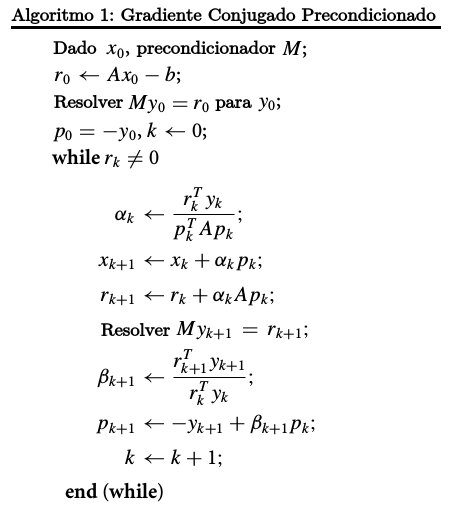
\includegraphics[width=0.45\textwidth]{GCPrec.png}
\caption*{}
\end{figure}

\subsection{Transformada de Fourier}

Para esta pr\'actica se implment\'o un precondicionador basado en la transformada de Fourier del sistema, utilizando la transformada discreta de Fourier en 2 dimensiones definida de la siguiente manera para una imagen de M X N:\\

$F(u,v)=\frac{1}{MN} \sum\limits_{x=0}^{M-1} \sum\limits_{y=0}^{N-1} f(x,y)e^{-2\pi i(\frac{ux}{M}+\frac{vy}{N})}$\\

y la transformada inversa de Fourier:\\

$f(x,y)=\frac{1}{MN} \sum\limits_{u=0}^{M-1} \sum\limits_{v=0}^{N-1} F(u,v)e^{-2\pi i(\frac{ux}{M}+\frac{vy}{N})}$\\

\section{Implementaci\'on}

Se implementan versiones de Gradiente Conjugado Lineal sin precondicionamiento y con precondicionamiento de Fourier. Con estas implementaciones se resuelve el problema de suavizamiento o "denoising" mediante la minimización de la función de regularizaci\'on definida por la siguiente expresión:\\

$U(I_1)=\frac{1}{2} \sum\limits_{x \in \Omega} (I_2(x)-I_1(x))^2+\frac{\lambda}{2} \sum\limits_{l \in N_x} \rho (I_1(x)-I_1(l))$\\

donde $N_x$ es la vecindad del pixel $I_1(x)$ de 4 vecinos, $\rho(z)=z^2$ es la función de regularizaci\'on con $z= I_1(x)-I_1(l)$, $I_1(x)$ es la imagen suavizada, $I_2(x)$ es la imagen observada con ruido, $x=(i,j)$ son las coordenadas de un pixel, $\Omega$ es el conjunto de pixeles en común a ambas imágenes y $\lambda$ es el parámetro de de regularizaci\'on o penalización.\\

Para maximizar la función definimos la derivada para cierto elemento $x_{ij}$:\\
 
$\frac{\partial}{\partial x_{ij}} U(I_1)=-[I_2(x_{ij})-I_1(x_{ij})]+\lambda \sum\limits_{l \in N_x} [I_1(x_{ij})-I_1(l)]$

Así generamos un sistema de ecuaciones para todo el dominio $\Omega$:\\

$I_1(x_{ij})[1+\lambda |N_x|]-\lambda \sum\limits_{l \in N_x} I_1(l)=I_2(x_{ij})$\\

donde $|N_x|$ representa el n\'umero de vecinos del pixel; en esta implementación estamos considerando un dominio continuo sobre la imagen, es decir, el vecino de un pixel en los extremos de la imagen, ser\'a el pixel del lado opuesto. Por tanto, cada pixel tendrá exactamente 4 vecinos.\\

\begin{figure}[hbtp]
\centering
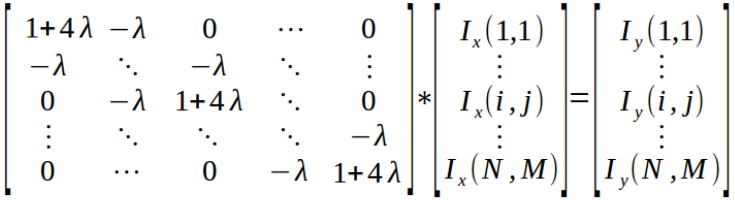
\includegraphics[width=0.45\textwidth]{system.png}
\caption*{}
\end{figure}

En este punto implementamos la transformada de Fourier como precondicionador en cada iteración del algoritmo de gradiente conjugado. Para cada renglón del sistema de ecuaciones tenemos que:\\

$\emph{\textbf{DFT}}[(1+4\lambda)I_1(x_{ij})-\lambda(I_1(x_{i-1,j})+I_1(x_{i+1,j})
+I_1(x_{i,j-1})+I_1(x_{i,j+1}))=I_2(x_{ij})]$\\

$\Rightarrow (1+4\lambda)F_{uv}-\lambda F_{uv}(e^{\frac{2\pi ui}{n}}+e^{\frac{-2\pi ui}{n}}+e^{\frac{2\pi vi}{n}}+e^{\frac{-2\pi vi}{n}})=G_{uv}$\\

y aplicamos la f\'ormula de Euler:\\

$e^{i\theta}+e^{-i\theta}=2 \cos \theta$\\

$\Rightarrow(1+4\lambda)F_{uv}-\lambda F_{uv}(2\cos(\frac{2\pi ui}{n})+2\cos(\frac{2\pi vi}{n}))=G_{uv}$\\

de esta manera obtenemos una expresión que nos permite resolver el sistema $F_{uv}=H_{uv}G_{uv}$ para $F_{uv}$:\\

$F_{uv}=\frac{1}{1+4 \lambda -2 \lambda(cos(\frac{2\pi ui}{n})+\cos(\frac{2\pi vi}{n}))}G_{uv}$\\

Esta f\'ormula es la que aplicaremos en cada paso de precondicionamiento, es decir, transformaremos el vector $g_{xy}$ a $G_{uv}$ en el dominio de Fourier y después de resolver para $F_{uv}$, transformaremos a $f_{xy}$ en el espacio cartesiano.\\


\section{Resultados}

A continuación se muestran las imágenes que se obtuvieron durante la ejecución de la práctica, para diferentes valores de $\lambda$ en una imagen de prueba:

\begin{figure}[hbtp]
\centering
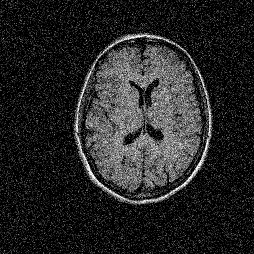
\includegraphics[width=0.35\textwidth]{mri.png}
\caption{Imagen observada}
\end{figure}

\begin{figure}[H]
	\centering
	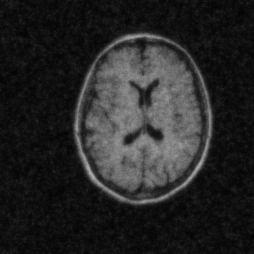
\includegraphics[width=0.15\textwidth]{ConjGrad2.png}
	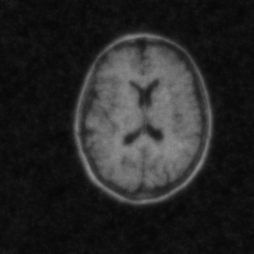
\includegraphics[width=0.15\textwidth]{ConjGrad5.png}
	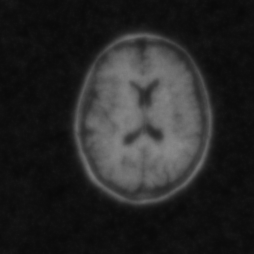
\includegraphics[width=0.15\textwidth]{ConjGrad10.png}
	
	\caption{De derecha a izquierda: Resultados de Gradiente Conjugado no precondicionado para $\lambda=2,5,10$, respectivamente.}
\end{figure}

\begin{figure}[H]
	\centering
	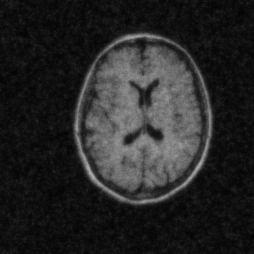
\includegraphics[width=0.15\textwidth]{FourierConjGrad2.png}
	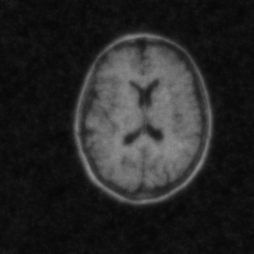
\includegraphics[width=0.15\textwidth]{FourierConjGrad5.png}
	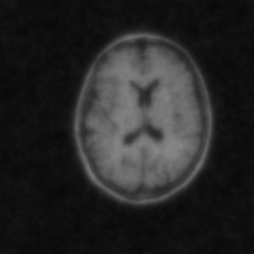
\includegraphics[width=0.15\textwidth]{FourierConjGrad10.png}
	
	\caption{De derecha a izquierda: Resultados de Gradiente Conjugado precondicionado con Transformada de Fourier para $\lambda=2,5,10$, respectivamente.}
\end{figure}

El programa implementado en esta práctica recibe el nombre del archivo de la imagen, el parámetro $\lambda$ y un indicador de la función a realizar, luego ejecuta los algoritmos de Gradiente Conjugado para suavizar la imagen con este parámetro.

Se imprime en pantalla el valor de $\lambda$, el tiempo de ejecución del algoritmo y el valor final de la función objetivo. Se muestra también una tabla donde se comparan ambos métodos con relación a su tiempo de ejecución, número de iteraciones y valor de la función objetivo:

\begin{figure}[hbtp]
\centering
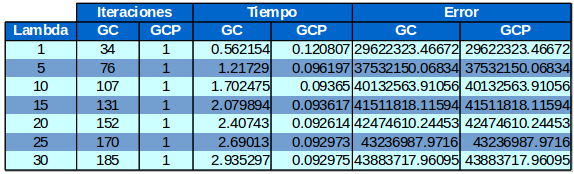
\includegraphics[width=0.5\textwidth]{tabla.png}
\caption{Tabla comparativa entre los algoritmo de Gradiente Conjugado implementados.}
\end{figure}

\section{Conclusiones}

Se observa por la tabla mostrada anteriormente que en general el algoritmo de Gradiente Conjugado con precondicionamiento de Fourier resulta ser m\'as eficiente, ya que siempre converge a una iteración puesto que estamos prácticamente resolviendo todo el sistema en el dominio de Fourier. Por otro lado en cuestión del valor de la función objetivo ambos arrojan resultados similares, lo cual se puede confirmar empíricamente al comparar las imágenes, ya que casi no muestran diferencias apreciables para una misma $\lambda$.

\bibliographystyle{plain}
\bibliography{biblio}


\appendix
\section{Implementation details}
El programa est\'a implementado tomando en cuenta todas estandarizaciones indicadas en el curso.

Un \textit{makefile} ha sido generado, el cual soporta los comandos \textit{make}, \textit{run} and \textit{clean}. El programa recibe como primer argumento el nombre del archivo de la imagen inicial, como segundo argumento el nombre del archivo de la imagen de referencia y por \'ultimo el indicador del método, 1 indica que se ejecutara Gradiente Conjugado sin precondicionamiento y 2 indica que se ejecutara con precondicionamiento.

\begin{figure}[hbtp]
\centering
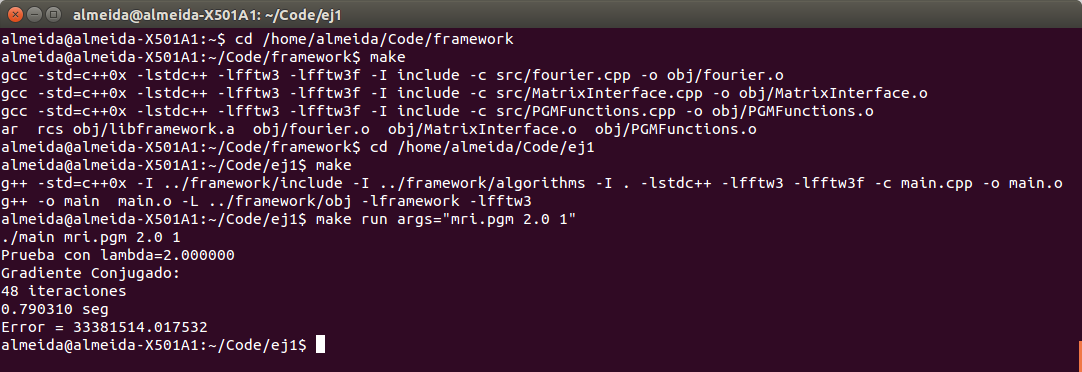
\includegraphics[width=0.5\textwidth]{screen.png}
\caption*{}
\end{figure}

\end{document}


